\documentclass[a4paper, 11pt]{article}
\usepackage{comment}
\usepackage{lipsum} 
\usepackage{fullpage} %cambiar margen
\usepackage[a4paper, total={7in, 10in}]{geometry}

\usepackage{amssymb,amsthm} 
\usepackage{amsmath}
\newtheorem{theorem}{Theorem}
\newtheorem{corollary}{Corollary}
\usepackage{graphicx}
\usepackage{tikz}
\usetikzlibrary{arrows}
\usepackage{verbatim}
%\usepackage[numbered]{mcode}
\usepackage{float}
\usepackage{tikz}
\usetikzlibrary{shapes,arrows}
\usetikzlibrary{arrows,calc,positioning}
\usepackage{mathpazo} %tipo de letra 
\usepackage[utf8]{inputenc} %codificación
\usepackage[T1]{fontenc} %digitación de tildes y ñ
\usepackage[spanish]{babel} %paquete de soporte español

\tikzset{
	block/.style = {draw, rectangle,
		minimum height=1cm,
		minimum width=1.5cm},
	input/.style = {coordinate,node distance=1cm},
	output/.style = {coordinate,node distance=4cm},
	arrow/.style={draw, -latex,node distance=2cm},
	pinstyle/.style = {pin edge={latex-, black,node distance=2cm}},
	sum/.style = {draw, circle, node distance=1cm},
}
\usepackage{xcolor}
\usepackage{mdframed}
\usepackage[shortlabels]{enumitem}
\usepackage{indentfirst}
\usepackage{hyperref}

\usepackage{listings}
\lstset{literate=
  {á}{{\'a}}1
  {é}{{\'e}}1
  {í}{{\'i}}1
  {ó}{{\'o}}1
  {ú}{{\'u}}1
  {Á}{{\'A}}1
  {É}{{\'E}}1
  {Í}{{\'I}}1
  {Ó}{{\'O}}1
  {Ú}{{\'U}}1
  {ñ}{{\~n}}1
  {ü}{{\"u}}1
  {Ü}{{\"U}}1
}

\lstdefinestyle{customc}{
  belowcaptionskip=1\baselineskip,
  breaklines=true,
  frame=L,
  xleftmargin=\parindent,
  language=Python,
  showstringspaces=false,
  basicstyle=\footnotesize\ttfamily,
  keywordstyle=\bfseries\color{green!40!black},
  commentstyle=\itshape\color{purple!40!black},
  identifierstyle=\color{blue},
  stringstyle=\color{orange},
}

\lstdefinestyle{customasm}{
  belowcaptionskip=1\baselineskip,
  frame=L,
  xleftmargin=\parindent,
  language=[x86masm]Assembler,
  basicstyle=\footnotesize\ttfamily,
  commentstyle=\itshape\color{purple!40!black},
}

\lstset{escapechar=@,style=customc}



\renewcommand{\thesubsection}{\thesection.\alph{subsection}}

\newenvironment{problem}[2][Ejercicio]
{ \begin{mdframed}[backgroundcolor= red!50] \textbf{#1 #2} \\}
	{  \end{mdframed}}

% Define solution environment
\newenvironment{solution}
{\textcolor{blue}{\textbf{\textit{Solución:\\\noindent}}}}


\renewcommand{\qed}{\quad\qedsymbol}

% \\	
\begin{document}
	\noindent
	%%%%%%%%%%%%%%%%%%%%%%%%%%%%%%%%%%%%
	
	\begin{minipage}[b][1.2cm][t]{0.8\textwidth}
		\large\textbf{César Isaí García Cornejo} \hfill \textbf{Tarea 4}  \\
		cesar.cornejo@cimat.mx \hfill \\
		\normalsize Computo Científico \hfill Semestre 3\\
	\end{minipage}
	
	\hspace{14.4cm}
	\begin{minipage}[b][0.03cm][t]{0.12\linewidth}
		
		\vspace{-2.2cm}
		%%%La Ruta dependera de donde este alojado el main y la imagen
		
\includegraphics[scale=0.3]{Figures/EscudoCimat.png}
	\end{minipage}
	
	\noindent\rule{7in}{2.8pt}
	
	%%%%%%%%%%%%%%%%%%%%%
	%%%%%%%%%%%%%%%%%%%%%%%%%%%%%%%%%%%%%%%%%%%%%%%%%%%%%%%%%%%%%%%%%%%%%%%%%%%%%%%%%%%%%%%%%%%%%%%%%%%%%%%%%%%%%%%%%%%
	% Problem 1
	%%%%%%%%%%%%%%%%%%%%%%%%%%%%%%%%%%%%%%%%%%%%%%%%%%%%%%%%%%%%%%%%%%%%%%%%%%%%%%%%%%%%%%%%%%%%%%%%%%%%%%%%%%%%%%%%%%%%%%%%%%%%%%%%%%%%%%%%
	\setlength{\parskip}{\medskipamount}
	\setlength{\parindent}{0pt}
%/////////// Ejercicio 1 /////////////////

\begin{problem}{1}
    Dado el siguiente

    \textit{Teorema (Gerschgorin):}

    \textit{Dada una matriz $A = a_{ij}$ de $m \times m$, cada eigenvalor de $A$ está en al menos uno de los discos en el plano complejo con centro en $a_{ii}$ y radio $\sum_{j\neq i }|a_{ij}|$. Además, si $n$ de estos discos forman un dominio conexo, disjunto de los otros $m-n$ discos, entonces hay exactamente $n$ eignevalores en ese dominio.}

    Deduce estimaciones de los eigenvalores de 
    \begin{align*}
        A = \begin{pmatrix}
            8 &1  &0 \\ 
             1&4  &\varepsilon \\ 
            0  &\varepsilon  &1 
            \end{pmatrix}
    \end{align*}
    con $|\varepsilon|<1$.

\end{problem}

\begin{solution}
    Veamos que por el Teorema de Gershgorin tenemos tres regiones disjuntas con centros dados por $8,4,1$, respectivamente. 
    Para la primer región $i=1$, tenemos un circulo en los complejos de centro 8 y radio 1. Para la segunda, región tenemos un circulo de centro 4 y radio $1 + \varepsilon $. Por último, para $i = 3$ tenemos un circulo de radio $\varepsilon$ y centro en 1.

    Con fines ilustrativos, la siguiente figura nos muestran las tres regiones en los complejos con un $\varepsilon$ arbitrario.

    \begin{figure}[H]
        \centering
        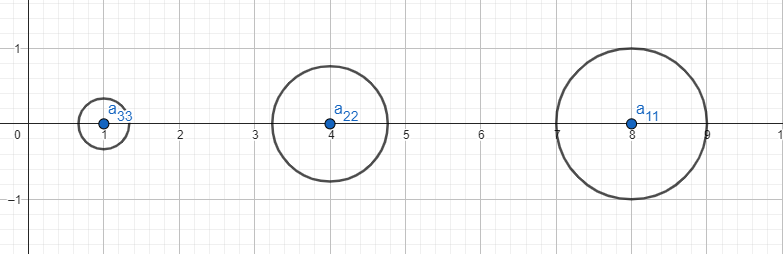
\includegraphics[width = 13 cm]{Figures/Gerschgorin.png}
        \caption{Regiones en el plano complejo donde cada región contiene un eigenvalor dado por el Teorema de Gerschgorin}
        \label{Fig. 01}
    \end{figure}

    Se puede observar además que la matriz $A$ es hermitiana. Por tanto, los eigenvalores de $A$ son reales. Luego, se puede acotar la estimación de los eigenvalores a la recta real, donde el eigenvalor máximo esta acotado superiormente por 9.

\end{solution}


\begin{problem}{2}
    Implementa la iteración QR con shift. Aplícala a la matriz $A$ del Ejercicio 1 con $\varepsilon = 10^{-N}$ para $N = 1,3,4,5.$
\end{problem}

\begin{solution} 


    Sabemos que el de iteración QR es un algoritmos que converge lentamente, en caso de que la matriz sea diagonalizable. Se puede mejorar la eficiencia en velocidad de convergencia implementando un \textit{shift} $\sigma$ en cada iteración. Hemos visto en clase que la convergencia del mencionado algoritmo depende del cociente $|\lambda_2/\lambda_1|$. Luego, se puede elegir un shift tal que
    \begin{align*}
        \frac{|\lambda_2-\sigma|}{|\lambda_1 - \sigma|} < \frac{|\lambda_2|}{|\lambda_1|}
    \end{align*}    
    Así, ajustando a cada iteración cierto \textit{shift} podemos mejorar la velocidad de convergencia.

    El construimos una función para el algoritmo de iteración QR para una matriz $A$


    \begin{verbatim}   
def diagonal(A,n):
    
    m = len(A)
    # Shift inicial
    sigma = A[m-1,m-1]
    
    T = A.copy()

    # n = 100           # Número de iteraciones
    for i in range(n):

        T = A - sigma*np.identity(m)
        Q, R = GramSchmidtModified(T)

        T = R@Q + sigma*np.identity(m)
        sigma =T[m-1,m-1]
    return T
    \end{verbatim}

La función retorna la matriz $T$ \textit{pseudo-diagonal}, que es la matriz $A$ tras $n$ iteraciones QR con \textit{shift.}

Construimos la matriz del problema 1, y en un ciclo buscamos la pseudo-diagonal para cada matriz simétrica.

Para la matriz
\begin{align*}
    \begin{bmatrix}
        8. & 1. & 0.\\
        1. & 4. & 1/10^N\\
        0. & 1/10^N & 1.\\
      \end{bmatrix}
\end{align*}
con 100 iteraciones QR se obtiene:

Caso $N=1$ 
\begin{align*}
    \begin{bmatrix}
        8.19994408e+00 & 4.00556947e-01 & 2.55849957e-01\\
        4.00556947e-01 & 3.80355156e+00 & 9.89997955e-02\\
        0.00000000e+00 & 1.79162876e-18 & 9.96504364e-01\\
      \end{bmatrix}
\end{align*}

Caso $N=3$
\begin{align*}
    \begin{bmatrix}
        8.19999999e+00 & 4.00000056e-01 & -4.76384063e-02\\
        4.00000056e-01 & 3.80000036e+00 & -5.94476093e-02\\
        0.00000000e+00 & 3.70934517e-21 & 9.99999650e-01\\
      \end{bmatrix}
\end{align*}

Caso $N=4$
\begin{align*}
    \begin{bmatrix}
        8.20000000e+00 & 4.00000001e-01 & 1.57892847e-03\\
        4.00000001e-01 & 3.80000000e+00 & 1.86170736e-03\\
        0.00000000e+00 & 1.38241560e-21 & 9.99999997e-01\\
      \end{bmatrix}
\end{align*}

Caso $N=5$
\begin{align*}
    \begin{bmatrix}
        8.20000000e+00 & 4.00000000e-01 & -5.15566331e-04\\
        4.00000000e-01 & 3.80000000e+00 & 9.89949491e-06\\
        0.00000000e+00 & 1.02401453e-23 & 1.00000000e+00\\
      \end{bmatrix}
\end{align*}

Notese que los elementos fuera de la diagonal son muy cercanos a cero. Vease que los elementos en la diagonal, que son los eignevalores, son aproximadamente de 8.2, 3.8, 1.

\end{solution}

\begin{problem}{3}
    Determina todos los eigenvalores y eigenvectores de una matriz de Householder.
\end{problem}

\begin{solution} 
Empecemos por definir la matriz de Householder.

\textbf{Definición}

Sea $v$ un vector columna de tamaño $k$. Se dice que la matriz de Householder asociada a $v$ es la matriz de dimensión $k \times k$ dada por
\begin{align*}
    H = I - 2 \frac{v v^*}{\left \| v \right \|^2}
\end{align*}
donde $I$ es la $k \times k$ matriz diagonal.

Dado esto, procederemos a mostrar que $H$ es hermitiana y unitaria.

\textbf{Teorema}

La matriz de Householder es hermitiana.

\textbf{Prueba}

Tomemos el transpuesto conjudado de $H$
\begin{align*}
    H^* &= I^* - 2 \frac{(vv^*)^*}{\left \| v \right \|^2},\\
    &= I - 2\frac{(v^*)^* v^*}{\left \| v \right \|^2},\\
    &= I - 2\frac{v v^*}{\left \| v \right \|^2} = H .
\end{align*}

\textbf{Teorema}

La matriz de Householder es unitaria.

\textbf{Prueba}

\begin{align*}
    HH^* &= H^2,\\ 
    &= \left(I - 2 \frac{v v^*}{\left \| v \right \|^2}\right)^2,\\
    &= I - 4\frac{v v^*}{\left \| v \right \|^2} +4 \frac{v v^*}{\left \| v \right \|^2}\frac{v v^*}{\left \| v \right \|^2},\\
    &= I -  4\frac{v v^*}{\left \| v \right \|^2} + 4\frac{v v^*}{\left \| v \right \|^2},\\
    &= I.
\end{align*}
donde se usó que $vv^* = \left \| v \right \|^2 $. 

Del hecho de que la matriz de Householder sea hermitiana se sigue que su valores propios existen y son reales. Por el hecho de que H sea unitaria significa que la tranformación generada en una rotación y/o reflexión. Entonces, los vectores propios deben estar en el circulo unitario. Por tanto, sus valores propios son $\pm 1$.

Para ver con formalidad el hecho previo. Tomemos
\begin{align*}
    Hv &= \left(I - 2 \frac{v v^*}{\left \| v \right \|^2}\right)v,\\
    &= v - 2 \frac{v (v^*v)}{\left \| v \right \|^2},\\
    &= v - 2 v,\\
    &= -v
\end{align*}
por lo que $v$ es vector propio con valor propio $-1$.

Ahora, consideremos un vector $u$ ortogonal al vector inicial $u$, es decir $v^*u = 0$. Entonces,
\begin{align*}
    Hu &= \left(I - 2 \frac{v v^*}{\left \| v \right \|^2}\right)u,\\
    &= u -2\frac{v (v^* u)}{\left \| v \right \|^2},\\
    &= u.
\end{align*}
como hay $k-1$ vectores ortogonales a $v$, se sigue que 1 es valor propio con multiplicidad $k-1$.



















\end{solution}


\begin{problem}{4}
    Demuestra que no es posible construir la tranformación de similaridad del Teorema de Schur con un número finito de tranformaciones de similaridad de Householder.
\end{problem}

\begin{problem}{5}
    ?` Qué pasa si aplicas la iteración QR sin shift a una matriz ortogonal? o \textbf{hagan lo que quieran}. Sea $A$ una matriz de Hessenberg superior y sea $QR = A$ la factorización QR de $A$. Muestra que $RQ$ es una matriz superior de Hessenberg.
\end{problem}










    \end{document}